\subsubsection{Caso d'uso UC8.2.4: Modifica domanda di collegamento}
\label{UC8.2.4}
\begin{figure}[ht]
	\centering
	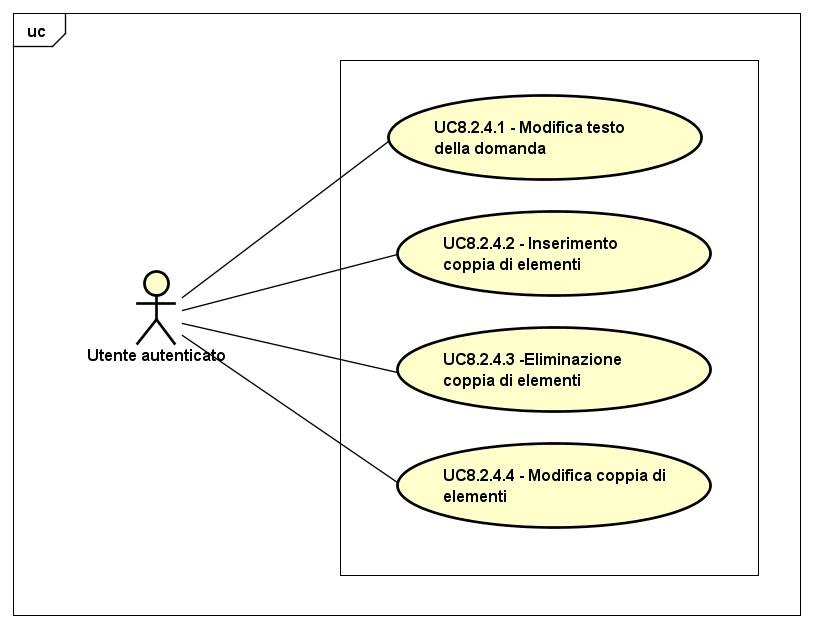
\includegraphics[scale=0.5,keepaspectratio]{UML/UC8_2_4.png}
	\caption{UC8.2.4: Modifica domanda di collegamento}
\end{figure}
\FloatBarrier
\begin{itemize}
	\item \textbf{Attori}: \uau, \uaupro;
	\item \textbf{Descrizione}: l'attore può utilizzare la procedura guidata per la modifica di una domanda di collegamento; 
	\item \textbf{Precondizione}: il sistema ha ricevuto dall'attore la domanda da modificare; 
	\item \textbf{Postcondizione}: l'attore ha modificato una domanda di collegamento;
	\item \textbf{Scenario principale}: 
	\begin{enumerate}
			\item L'attore può modificare il testo della domanda (UC8.2.4.1);
			\item L'attore può inserire una coppia di elementi (UC8.2.4.2);
			\item L'attore può eliminare una coppia di elementi inserita (UC8.2.4.3);
			\item L'attore può modificare una coppia di elementi inserita (UC8.2.4.4).
		\end{enumerate}
	\item \textbf{Scenari alternativi}: se non ci sono almeno due coppie presenti nella lista delle coppie l'attore deve inserire una nuova coppia di elementi.
\end{itemize}

	\subsubsection{Caso d'uso UC8.2.4.1: Modifica testo della domanda}
	\label{UC8.2.4.1}
	\begin{itemize}
		\item
		\textbf{Attori}: \uau, \uaupro;
		\item		
		\textbf{Descrizione}: l'attore può modificare il testo della domanda;
		\item
		\textbf{Precondizione}: il sistema mostra la funzionalità di modifica di una domanda di collegamento; 
		\item
		\textbf{Postcondizione}: l'attore ha modificato il testo della domanda;
		\item
		\textbf{Scenario principale}: l'attore modifica il testo della domanda.	
	\end{itemize}

	\subsubsection{Caso d'uso UC8.2.4.2: Inserimento coppia di elementi}
	\label{UC8.2.4.2}
	\begin{figure}[h]
		\centering
		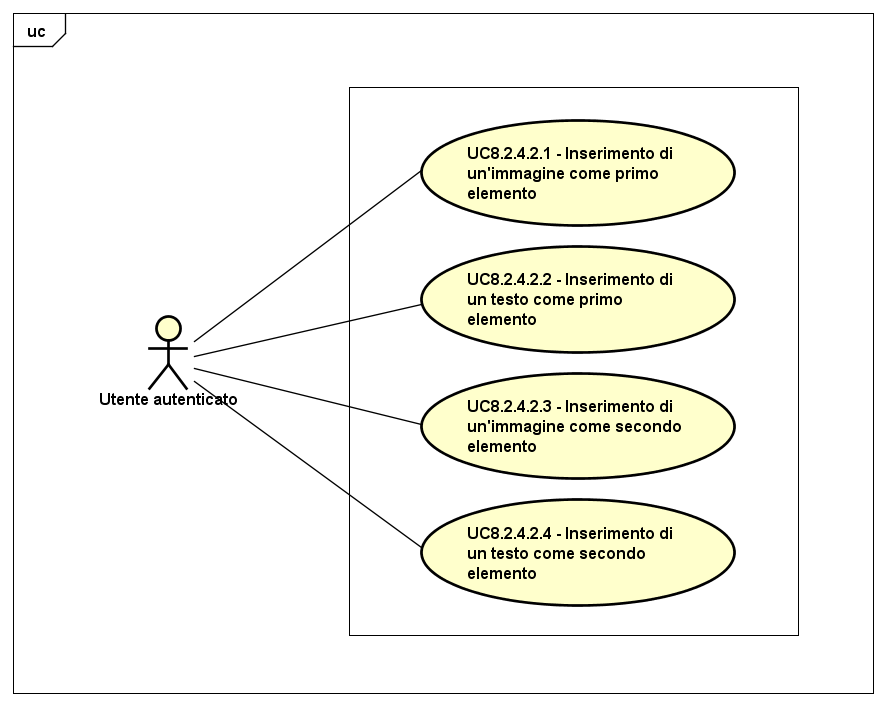
\includegraphics[scale=0.5,keepaspectratio]{UML/UC8_2_4_2.png}
		\caption{UC8.2.4.2: Inserimento coppia di elementi}
	\end{figure}
	\FloatBarrier
	\begin{itemize}
		\item \textbf{Attori}: \uau, \uaupro;
		\item \textbf{Descrizione}: l'attore può inserire una coppia di elementi, sia immagini che testo o combinazioni di questi, che siano correlati tra loro in modo da indicare la soluzione della domanda; 
		\item \textbf{Precondizione}: il sistema mostra la funzionalità di modifica di una domanda di collegamento; 
		\item \textbf{Postcondizione}: l'attore ha inserito una coppia di elementi nella lista di coppie di elementi; 
		\item \textbf{Scenario principale}: 
		\begin{enumerate}
			\item L'attore inserisce come primo elemento un'immagine (UC8.2.4.2.1);
			\item L'attore inserisce come primo elemento un testo (UC8.2.4.2.2);
			\item L'attore inserisce come secondo elemento un'immagine (UC8.2.4.2.3);
			\item L'attore inserisce come secondo elemento un testo (UC8.2.4.2.4).	
		\end{enumerate}
	\end{itemize}
	
		\subsubsection{Caso d'uso UC8.2.4.2.1: Inserimento di un'immagine come primo elemento}
		\label{UC8.2.4.2.1}
		\begin{itemize}
			\item \textbf{Attori}: \uau, \uaupro;
			\item \textbf{Descrizione}: l'attore può inserire come primo elemento della coppia un'immagine;
			\item \textbf{Precondizione}: il sistema mostra la funzionalità di modifica di una domanda di collegamento; 
			\item \textbf{Postcondizione}: l'attore ha inserito come primo elemento un'immagine;
			\item \textbf{Scenario principale}: l'attore carica un'immagine come primo elemento della coppia.
		\end{itemize}
		
		\subsubsection{Caso d'uso UC8.2.4.2.2: Inserimento di un testo come primo elemento}
		\label{UC8.2.4.2.2}
		\begin{itemize}
			\item \textbf{Attori}: \uau, \uaupro;
			\item \textbf{Descrizione}: l'attore può inserire come primo elemento della coppia un testo;
			\item \textbf{Precondizione}: il sistema mostra la funzionalità di modifica di una domanda di collegamento; 
			\item \textbf{Postcondizione}: l'attore ha inserito come primo elemento un testo;
			\item \textbf{Scenario principale}: l'attore inserisce del testo come primo elemento della coppia.
		\end{itemize}
		
			\subsubsection{Caso d'uso UC8.2.4.2.3: Inserimento di un'immagine come secondo elemento}
		\label{UC8.2.4.2.3}
		\begin{itemize}
			\item \textbf{Attori}: \uau, \uaupro;
			\item \textbf{Descrizione}: l'attore può inserire come secondo elemento della coppia un'immagine;
			\item \textbf{Precondizione}: il sistema mostra la funzionalità di modifica di una domanda di collegamento; 
			\item \textbf{Postcondizione}: l'attore ha inserito come secondo elemento un'immagine;
			\item \textbf{Scenario principale}: l'attore carica un'immagine come secondo elemento della coppia.
		\end{itemize}
		
		\subsubsection{Caso d'uso UC8.2.4.2.4: Inserimento di un testo come secondo elemento}
		\label{UC8.2.4.2.4}
		\begin{itemize}
			\item \textbf{Attori}: \uau, \uaupro;
			\item \textbf{Descrizione}: l'attore può inserire come secondo elemento della coppia un testo;
			\item \textbf{Precondizione}:il sistema mostra la funzionalità di modifica di una domanda di collegamento; 
			\item \textbf{Postcondizione}: l'attore ha inserito come secondo elemento un testo;
			\item \textbf{Scenario principale}: l'attore inserisce del testo come secondo elemento della coppia.
		\end{itemize}
	
	\subsubsection{Caso d'uso UC8.2.4.3: Eliminazione coppia di elementi}
	\label{UC8.2.4.3}
	\begin{figure}[h]
		\centering
		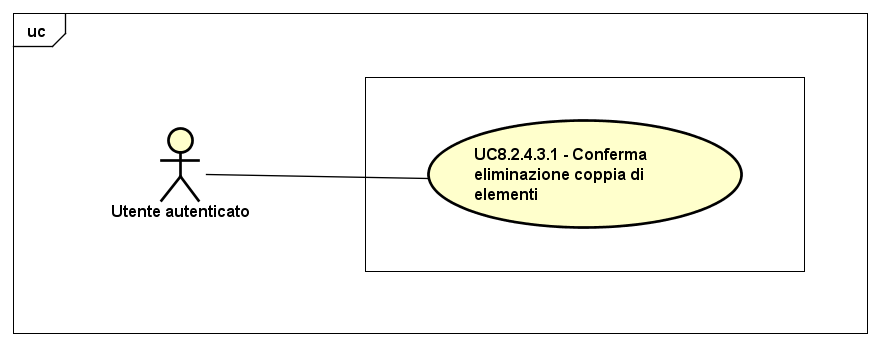
\includegraphics[scale=0.5,keepaspectratio]{UML/UC8_2_4_3.png}
		\caption{UC8.2.4.3: Eliminazione coppia di elementi}
	\end{figure}
	\FloatBarrier
	\begin{itemize}
		\item \textbf{Attori}: \uau, \uaupro;
		\item \textbf{Descrizione}: l'attore può rimuovere una coppia di elementi dalla lista di coppie di elementi;
		\item \textbf{Precondizione}: il sistema mostra la funzionalità di modifica di una domanda di collegamento; 
		\item \textbf{Postcondizione}: l'attore ha eliminato una coppia di elementi dalla lista delle coppie di elementi;
		\item \textbf{Scenario principale}: l'attore può confermare l'eliminazione di una coppia di elementi (UC8.2.4.3.1);
		\item \textbf{Scenari alternativi}: l'attore annulla l'operazione tornando alla schermata precedente.
	\end{itemize}

		\subsubsection{Caso d'uso UC8.2.4.3.1: Conferma eliminazione coppia di elementi}
		\label{UC8.2.4.3.1}
		\begin{itemize}
			\item \textbf{Attori}: \uau, \uaupro;
			\item \textbf{Descrizione}: l'attore può confermare la rimozione di una coppia di elementi;
			\item \textbf{Precondizione}: il sistema mostra la funzionalità di modifica di una domanda di collegamento; 
			\item \textbf{Postcondizione}: l'attore ha confermato l'eliminazione della coppia di elementi;
			\item \textbf{Scenario principale}: l'attore conferma la rimozione della coppia di elementi.
		\end{itemize}

	\subsubsection{Caso d'uso UC8.2.4.4: Modifica coppia di elementi}
	\label{UC8.2.4.4}
	\begin{figure}[h]
		\centering
		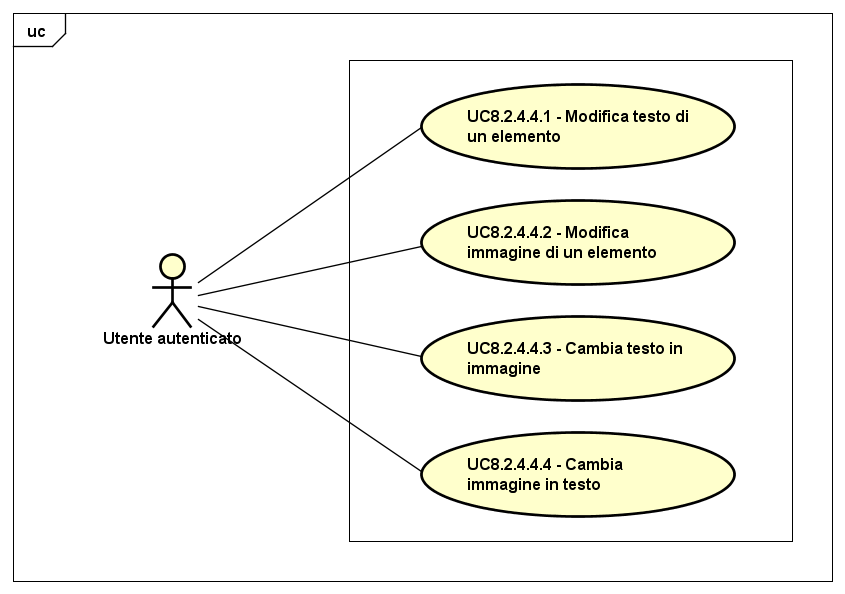
\includegraphics[scale=0.5,keepaspectratio]{UML/UC8_2_4_4.png}
		\caption{UC8.2.4.4: Modifica coppia di elementi}
	\end{figure}
	\FloatBarrier
	\begin{itemize}
		\item \textbf{Attori}: \uau, \uaupro;
		\item \textbf{Descrizione}: l'attore può modificare una coppia di elementi presente nella lista di coppie di elementi;
		\item \textbf{Precondizione}: il sistema mostra la funzionalità di modifica di una domanda di collegamento; 
		\item \textbf{Postcondizione}: l'attore ha modificato una coppia di elementi presente nella lista di coppie di elementi; 
		\item \textbf{Scenario principale}: 
		\begin{enumerate}
			\item L'attore può modificare un elemento cambiandone il testo (UC8.2.4.4.1);
			\item L'attore può modificare un elemento cambiandone l'immagine (UC8.2.4.4.2);
			\item L'attore può modificare un elemento facendolo passare da testo ad immagine (UC8.2.4.4.3);
			\item L'attore può modificare un elemento facendolo passare da immagine a testo (UC8.2.4.4.4).	
		\end{enumerate}
	\end{itemize}
	
		\subsubsection{Caso d'uso UC8.2.4.4.1: Modifica testo di un elemento}
		\label{UC8.2.4.4.1}
		\begin{itemize}
			\item \textbf{Attori}: \uau, \uaupro;
			\item \textbf{Descrizione}: l'attore può modificare il testo di un elemento;
			\item \textbf{Precondizione}: il sistema mostra la funzionalità di modifica di una domanda di collegamento; 
			\item \textbf{Postcondizione}: l'attore ha modificato il testo di un elemento;
			\item \textbf{Scenario principale}: l'attore modifica il testo di un elemento.  
		\end{itemize}
		
		\subsubsection{Caso d'uso UC8.2.4.4.2: Modifica immagine di un elemento}
		\label{UC8.2.4.4.2}
		\begin{itemize}
			\item \textbf{Attori}: \uau, \uaupro;
			\item \textbf{Descrizione}: l'attore può caricare un'altra immagine per un elemento;
			\item \textbf{Precondizione}: il sistema mostra la funzionalità di modifica di una domanda di collegamento; 
			\item \textbf{Postcondizione}: l'attore ha inserito un'altra immagine per un elemento;
			\item \textbf{Scenario principale}: l'attore carica un'altra immagine per un elemento.
		\end{itemize}
		
		\subsubsection{Caso d'uso UC8.2.4.4.3: Cambia testo in immagine}
		\label{UC8.2.4.4.3}
		\begin{itemize}
			\item \textbf{Attori}: \uau, \uaupro;
			\item \textbf{Descrizione}: l'attore può modificare un elemento facendolo diventare un'immagine al posto di un testo;
			\item \textbf{Precondizione}: il sistema mostra la funzionalità di modifica di una domanda di collegamento; 
			\item \textbf{Postcondizione}: l'attore ha fatto diventare un'immagine un elemento che prima era un testo;
			\item \textbf{Scenario principale}: l'attore inserisce un'immagine come modifica dell'elemento.  
		\end{itemize}
		
		\subsubsection{Caso d'uso UC8.2.4.4.4: Cambia immagine in testo}
		\label{UC8.2.4.4.4}
		\begin{itemize}
			\item \textbf{Attori}: \uau, \uaupro;
			\item \textbf{Descrizione}: l'attore può modificare un elemento facendolo diventare un testo al posto di un'immagine;
			\item \textbf{Precondizione}: il sistema mostra la funzionalità di modifica di una domanda di collegamento; 
			\item \textbf{Postcondizione}: l'attore ha fatto diventare un testo un elemento che prima era un'immagine;
			\item \textbf{Scenario principale}: l'attore inserisce del testo come modifica dell'elemento.  
		\end{itemize}